
\documentclass{article}
\title{Sailor GSoC Report}
\date{May 25th 2015}
\author{Etiene Dalcol}
\usepackage[T1]{fontenc}
\usepackage[backend=bibtex,style=verbose-trad2]{biblatex}
\usepackage{graphicx}
\usepackage[a4paper, total={6in, 8in}]{geometry}       
\bibliography{main} 
\begin{document}
	\pagenumbering{gobble}

\begin{titlepage}

\newcommand{\HRule}{\rule{\linewidth}{0.5mm}} % Defines a new command for the horizontal lines, change thickness here

\center % Center everything on the page
 
%----------------------------------------------------------------------------------------
%	HEADING SECTIONS
%----------------------------------------------------------------------------------------

\textsc{\LARGE �cole Nationale Sup�rieure de Techniques Avanc�es Bretagne}\\[0.5cm] % Name of your university/college

\includegraphics[scale=0.15]{enstalogo.jpg}\\[0.5cm]
\textsc{\Large Summer Internship Report}\\[0.5cm] % Major heading such as course name
\textsc{\large Web development in Lua programming language}\\[0.5cm] % Minor heading such as course title

%----------------------------------------------------------------------------------------
%	TITLE SECTION
%----------------------------------------------------------------------------------------

\HRule \\[0.4cm]
{ \huge \bfseries Improvements to Sailor framework during Google Summer of Code}\\[0.4cm] % Title of your document
\HRule \\[0.5cm]



\includegraphics[scale=0.15]{logo-lua.png}

\includegraphics[scale=0.3]{gsoclogo.jpg}\\[1.5cm]
 
%----------------------------------------------------------------------------------------
%	AUTHOR SECTION
%----------------------------------------------------------------------------------------

\begin{minipage}{0.4\textwidth}
\begin{flushleft} \large
\emph{Author:}\\
Etiene \textsc{da Cruz Dalcol} % Your name
\end{flushleft}
\end{minipage}
~
\begin{minipage}{0.4\textwidth}
\begin{flushright} \large
\emph{Supervisor:} \\
Dr. Olivier \textsc{Reynet} % Supervisor's Name
\end{flushright}
\end{minipage}\\[1.5cm]

% If you don't want a supervisor, uncomment the two lines below and remove the section above
%\Large \emph{Author:}\\
%John \textsc{Smith}\\[3cm] % Your name

%----------------------------------------------------------------------------------------
%	DATE SECTION
%----------------------------------------------------------------------------------------

{\large \today}\\[3cm] % Date, change the \today to a set date if you want to be precise

%----------------------------------------------------------------------------------------
%	LOGO SECTION
%----------------------------------------------------------------------------------------


% Include a department/university logo - this will require the graphicx package


 
%----------------------------------------------------------------------------------------

\vfill % Fill the rest of the page with whitespace

\end{titlepage}




	\newpage
	\tableofcontents

	\newpage
	\pagenumbering{arabic}

	\section{Abstract}

Lua is a very fast and powerful scripting language that can be easily embeddable. For that reason, it has gained a niche in the game development industry. Lua has great potential and incredible benchmarks. Despite being also an excellent tool as a general purpose language to develop robust applications, its use in web developments needs to be more widespread. \\

Sailor was invented to increase the ecosystem of web development in Lua but it is still in early development. The purpose of this work is to turn Sailor into a more mature software by adding new features and improving existing ones such as adding automated tests and improving the use of Lua instead of Javascript when programming for the browser. 

	\subsection*{Resum�}\\
Lua est un langage tr�s rapide et puissant qui peut �tre embarqu� facilement. Pour cette raison, il a gagn� une place importante dans l'industrie de d�veloppement de jeux. Lua a des potentiels et benchmarks incroyables. En d�pit d'�tre aussi un excellent outil en tant que langue d'usage g�n�ral pour d�velopper des applications robustes, son utilisation dans le d�veloppement web devrait �tre plus g�n�ralis�e.\\

Sailor a �t� invent� pour augmenter l'�cosyst�me du d�veloppement web en Lua, mais il est encore dans un stage de d�veloppement pr�coce. Le but de ce travail est de transformer Sailor dans un logiciel plus mature en ajoutant de nouvelles fonctionnalit�s et l'am�lioration de ceux existants, tels que l'ajout de tests automatis�s et d'am�lioration de l'utilisation de Lua lieu de Javascript lors de la programmation pour le navigateur.


	\newpage
	
	\section{Introduction}

	\subsection{Google Summer of Code}
	Google Summer of Code (GSoC) is a global program that connects students with open source, free software and technology-related organizations. During the a 3 month period on the summer, the students get familiarised with open source projects, work with the community and write code. \\

Google identifies open source projects and organizations that will receive funding and participate on the program. The organizations will provide mentors to guide students during the program. Students submit projects to the organizations, who rank them. Organizations may suggest a list of ideas for projects. Once Google defines how many student slots for projects are allocated to an organization, the organization decides which students and projects are accepted and pair them with a mentor.\\

While most students come from a Computer Science and Software Engineering background, this is not mandatory and the educational area of participants can be very wide.\\

The program is centered on some goals\autocite{gsocgoals}:
\begin{quote}\begin{enumerate}\item Get more open source code written and released for the benefit of all.
\item Inspire young developers to begin participating in open source development.
\item Help open source projects identify and bring in new developers.
\item Provide students the opportunity to do work related to their academic pursuits during the summer: "flip bits, not burgers."
\item Give students more exposure to real-world software development (for example, distributed development and version control, software licensing issues, and mailing list etiquette)."
	\end{enumerate}
\end{quote}

There are midterm and final evaluations, and the code completed must be submitted to GSoC's website by the end of the program. All development happens online, Google does not provide an office space and there's no requirement to travel.\\

Since the start of the program, in 2005, over 8500 successful students have participated, from over 109 countries, with 8000 mentors making 55 million lines of code.


\subsection{LabLua}
	
LabLua was one of the organizations selected to participate in the 2015 version of Google Summer of Code. It is a research lab at the Pontifical Catholic University of Rio de Janeiro (PUC-Rio) affiliated with its Computer Science Department. Its researches are on the field of programming languages, with an emphasis on the Lua programming language. The founder of LabLua, Prof. Roberto Ierusalimschy, is one of the creators of the Lua language.\\

LabLua proposed the following list of ideas to GSoC: 

\begin{enumerate}\item LuaRocks add-ons system
\item Port Lua Test Suite to NetBSD Kernel
\item Elasticsearch Lua client (elasticsearch-lua)
\item Add support for left recursion to LPeg
\item Switch Typed Lua from optional typing to gradual typing
\item Adapt CGILua SAPI launcher to explore all WSAPI features
\item Add support for WSDL generation to LuaSOAP
\item Add support for prepared statements in LuaSQL
\item Multi-CPU usage in VLC
\item Multi-CPU usage in wireshark
\item Develop a binary serialization format with support for dynamically types values and an RPC protocol for dynamically typed invocations based on this format.
\item Develop a library for Lua that allows Lua programs to access features provided by the platform's underlying operating system (OS) kernel, such as process control, network access, file system, event notification, etc.
\item Port an SDL-based C++ open source game to C�u
\end{enumerate}

They received in total 6 slots, from which, four of them were filled by students working on ideas 2, 3, 7 and 13 and two of them were ideas proposed by students themselves. One of the student-proposed ideas was my project to improve Sailor, a web development framework I had been developing on my free time. \\

The project was mentored by Dr. Fabio Mascarenhas, professor at Universidade Federal do Rio de Janeiro. Since Google did not provide for office space or work placement, ENSTA Bretagne offered a placement during the summer to work on this project under the supervision of Professor Dr. Olivier Reynet. \\

\subsection{The Lua programming language}

\begin{quotation}Lua is a powerful, fast, lightweight, embeddable scripting language.\autocite{luaorg}\end{quotation}

This description provided by lua.org does not fully grasp what's interesting about this language. Lua was created in a very specific context: Petrobras, a multinational energy and oil corporation headquartered in Rio de Janeiro, Brazil had interactive graphical programs for engineering applications. These programs needed some flexibility and they were used by non professional programmers. Lua was created to be very simple yet powerful, allowing the customisation of these softwares through scripting. Avoiding cryptic syntax and semantics, Lua is a very readable language with a short learning curve. \\

It's possible to have an idea about the simplicity of this language just by comparing the brevity of the Programming in Lua book versus books on pretty much any other language. This means you can have all of the language in your head. Its source code is also very succinct. As of version 5.3.1, described in about 23000 lines of Standard C, the whole distribution which includes documentation has only 276Kb. This allows easily porting Lua code to things that run standard ANSI C, even if they have typically low resources, and embedding Lua to applications without bloating them. The result is that Lua is a very widely used language, from micro controllers and washing machines to operating systems, power computers and video games.\\

Its power can be observed on its multi-paradigm extensible semantics and speed. For example, while Lua does not come with Object Oriented Programming out of the box, it is possible to prototype it using first class functions \footnote{Support of passing functions as arguments to other functions, returning them as the values from other functions, and assigning them to variables or storing them in data structures. \autocite{wikifunc}} and metatables \footnote{Allows to change the behavior of a table. It is part of an extension mechanism which allows you to overload certain operations on Lua objects. \autocite{luausersmeta} \autocite[117]{pil}}. Lua also performs way better than other popular programming languages on speed tests. A special dialect of Lua called LuaJIT is the fastest it can get while still being a dynamically typed scripting language\autocite[8]{modlua}: \\

%\clearpage
\begin{figure}[h]
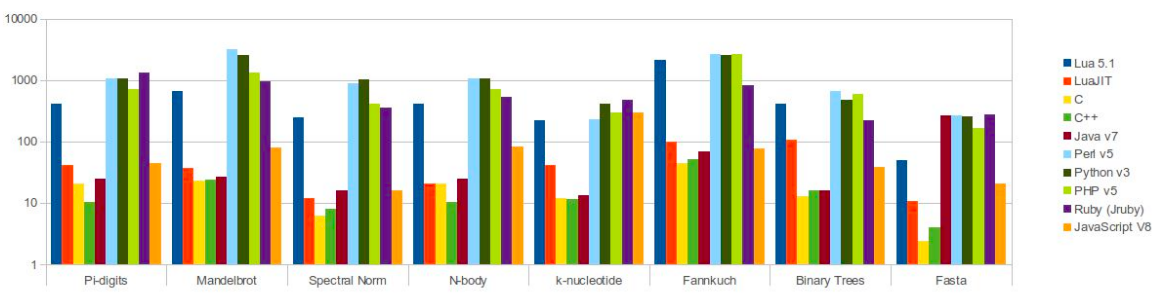
\includegraphics[scale=0.4]{speed.png}
\caption{\label{fig:speedcomparison} Speed comparison of popular script languages (less is better)}
\end{figure}



		\subsection{Schedule}

		\begin{description}
	  \item[May 25th - June 5th] \hfill \\
	  Researching how other frameworks use their test suites
	  \item[June 6th - June 15th] \hfill \\
	  Researching and testing existent test Lua modules
	  \item[June 16th - July 1st] \hfill \\
	  Either integrating an existing test module with Sailor or developing a new one
	  \item[July 2nd - July 16th] \hfill \\
	  Testing, bug fixing and documenting
			\item[July 17th - July 23rd] \hfill \\
	  Researching and testing Lua to JavaScript VMs. E.g. MoonshineJS
			\item[July 24th - August 6th] \hfill \\
	  Improving current way to manipulate DOM from Lua and load Lua modules to be used on client side.
			\item[August 7th - August 16th] \hfill \\
	  Testing, bug fixing and documenting
			\item[August 17th - August 21st] \hfill \\
	  Polishing and making sure nothing was missed
		\end{description}
		
	\section{Section}
		\subsection{Subsection}

			Structuring a document is easy! \autocite[97]{johnsbook}

		\subsubsection{Subsubsection}

			More text. \autocite{VELLAGE:1}

			\paragraph{Paragraph}

				Some more text. \\ %linebreak

				\subparagraph{Subparagraph}

					Even more text.

	\newpage
	\section{Another section}

	\newpage

%\printbibliography
%\printbibheading[title={References},heading=bibnumbered]
\section{References}
	\printbibliography[title={Books},type=book,heading=subbibnumbered]
	\printbibliography[title={Articles},type=article,heading=subbibnumbered]
	\printbibliography[title={Websites},type=misc,heading=subbibnumbered]

	\newpage
	\section{Appendix}
	\begin{appendix}
	%\addcontentsline{toc}{subsection}{List of Figures}
	 \listoffigures
	 % \addcontentsline{toc}{subsection}{List of Tables}
  \listoftables
	\end{appendix}

\end{document}